\documentclass[%
reprint,
superscriptaddress,
%groupedaddress,
%unsortedaddress,
%runinaddress,
%frontmatterverbose,
%preprint,
showpacs,preprintnumbers,
%nofootinbib,
%nobibnotes,
%bibnotes,
amsmath,amssymb,
aps,
%pra,
%prb,
prd,
%prl,
%rmp,
%prstab,
%prstper,
%floatfix,
]{revtex4-1}

\usepackage{float}
\usepackage{graphicx}% Include figure files
\usepackage{dcolumn}% Align table columns on decimal point
\usepackage{bm}% bold math
\usepackage{bbold}
\usepackage{braket}
\usepackage{amssymb,amsmath}


\usepackage{color}
%\usepackage[dvipsnames, svgnames, x11names]{xcolor}
\usepackage{amsfonts}
\usepackage{subfigure}
\usepackage{array}


\newcommand{\Tr}{\ensuremath{\operatorname{Tr}}}
\newcommand{\tr}{\ensuremath{\operatorname{tr}}}
\newcommand{\Omegaqq}{\ensuremath{\Omega_{\bar{q}q}}}
\newcommand{\vev}[1]{\ensuremath{\left\langle #1 \right\rangle}}
\newcommand{\einh}[1]{\ensuremath{\,\text{#1}}}
\newcolumntype{L}{>{\centering\arraybackslash}m{3cm}}



\newcommand{\overbar}[1]{\mkern 1.5mu\overline{\mkern-1.5mu#1\mkern-1.5mu}\mkern 1.5mu}



% color def's

\definecolor{blue}{rgb}{0,0,1}
\newcommand{\colb}[1]{{\color{blue} #1}}
\definecolor{green}{rgb}{0,1,0}
\newcommand{\colg}[1]{{\color{green} #1}}
\definecolor{red}{rgb}{1,0,0}
\newcommand{\colr}[1]{{\color{red} #1}}
\newcommand{\colJ}[1]{{\color{cyan} #1}}
\definecolor{gray}{rgb}{.5,.5,.5}
\newcommand{\drop}[1]{{\sout{ {\color{gray} #1}}}}
\definecolor{darkgreen}{rgb}{.0,.5,.0}
\newcommand{\colL}[1]{{\color{darkgreen} #1}}


% units and refs
\usepackage{xspace}
\usepackage{siunitx}
\usepackage{xfrac}
\usepackage{hyperref}
\usepackage[nameinlink]{cleveref}
\usepackage{appendix}
\usepackage{units}
% other
\usepackage{xifthen}
\usepackage{xcolor}
\hypersetup{
	colorlinks,
	linkcolor={red!75!black},
	citecolor={blue!75!black},
	urlcolor={blue!75!black}
}
%%%%%%%%%%%%%%% Refs %%%%%%%%%%%%%%%%%%%%%%%%%%%
\def\Fig#1{\Cref{#1}}
\def\Figs#1{\Cref{#1}}
\def\fig#1{\Cref{#1}}

\def\Tab#1{\Cref{#1}}
\def\tab#1{\Cref{#1}}

\def\Eqs#1{\Cref{#1}}
\def\Eq#1{\Cref{#1}}
\def\eq#1{\Cref{#1}}
\def\eqref#1{\Cref{#1}}

\def\sec#1{\Cref{#1}}
\def\app#1{\hyperref[#1]{App.~\ref{#1}}}
\def\app#1{\Cref{#1}}

\renewcommand{\tableautorefname}{Tab.}
\renewcommand{\equationautorefname}{Eq.}
%%%%%%%%%%%%%%%%%%%%%%%%%%%%%%%%%%%%%%%%

\newcommand{\Phibar}{\ensuremath{\bar{\Phi}}}
\newcommand{\LPQM}{\ensuremath{\mathcal{L}_{\textrm{PQM}}}\xspace}

\def\dbar{{\mathchar'26\mkern-12mu d}}
\def\lA0{{\langle A_0 \rangle}}
\def\bA0{{\bar{A}_0}}
\def\lLA{{\langle L[A_0] \rangle}}
\def\lL{{\langle L \rangle}}
\def\lLc{{\langle L^\dagger \rangle}}
\def\lLAc{{\langle L^\dagger[A_0] \rangle}}


\def\dr{{D\!\llap{/}}\,}
\def\Dr{{D\!\llap{/}}\,}
\def\ipv{\vec{p}\llap{/}}
\def\pslash{p\llap{/}}

\def\0#1#2{\frac{#1}{#2}}

\newcommand{\bsig}{\ensuremath{\bar{\sigma}}}
\newcommand{\lsm}{L\ensuremath{\sigma}M\xspace}
\newcommand{\pT}{\ensuremath{T_0}}
\newcommand{\Tl}{\ensuremath{T_\chi}}
\newcommand{\Ts}{\ensuremath{T_\chi^s}}
\newcommand{\Tchi}{\ensuremath{T_\chi}}
\newcommand{\Td}{\ensuremath{T_d}}
\newcommand{\Tc}{\ensuremath{T_c}}
\newcommand{\muc}{\ensuremath{\mu_c}}
\newcommand{\coloronl}{(color online)\xspace}

\newcommand{\mrm}[1]{\mathrm{#1}}
\def\qbar{\bar{q}}
\newcommand{\sx}{\sigma_{x}}
\newcommand{\sy}{\sigma_{y}}

%%%%%%%%%%%%% Hypersetup %%%%%%%%%%%%%

\newcommand{\gettitle}{Baryon number fluctuations at finite temperature and density in QCD}

\renewcommand{\figureautorefname}{Fig.}
\renewcommand{\sectionautorefname}{Sec.}
\renewcommand{\subsectionautorefname}{Subsec.}
\renewcommand*{\appendixautorefname}{App.}


%%%%%%%%%%%%%% for corrections %%%%%%%%%%%
\newcommand{\colwj}[1]{\textcolor{blue}{#1}}
\newcommand{\cJMP}[1]{\textcolor{red}{#1}}
\newcommand{\colfab}[1]{\textcolor{magenta}{#1}}
\newcommand{\colrui}[1]{\textcolor{green}{#1}}
\newcommand{\colshi}[1]{\textcolor{Plum}{#1}}

%
%%%%%%%%%%%%%%%%%%%%%%%%%%%%%%%%%%%%%%%%%%%%%%%%%%%%%%%%%%%%%%%%%%%%%%%%%%%%%

\graphicspath{{./figures/}{./}}

\begin{document}
%\preprint{}
	
\title{Equation of state and baryon number fluctuations at finite temperature and density in QCD}
	
	

\author{Wei-jie Fu}
\affiliation{School of Physics, Dalian University of Technology, Dalian, 116024,
		P.R. China}

\author{Jan M. Pawlowski}
\affiliation{Institut f\"ur Theoretische Physik, Universit\"at Heidelberg, Philosophenweg 16, 69120 Heidelberg, Germany}
	\affiliation{ExtreMe Matter Institute EMMI, GSI, Planckstra{\ss}e 1, D-64291 Darmstadt, Germany}
	
\author{Fabian Rennecke}
\affiliation{Brookhaven National Laboratory, Upton, NY 11973, USA}
	
\author{Rui Wen}
\affiliation{School of Physics, Dalian University of Technology, Dalian, 116024,
		P.R. China}
	
\author{Shi Yin}
\affiliation{School of Physics, Dalian University of Technology, Dalian, 116024,
		P.R. China}
	
	
\begin{abstract}
This paper is a further work of \cite{Fu:2019hdw}. We improve the $N_f=2+1$ QCD theory within the functional renormalization group (FRG) approach at finite temperature and baryon chemical potential. Starting from the gluon and quark degrees of freedom in the perturbative high-energy regime,  we systematically integrate out quantum fluctuations towards the mesons and baryons degrees of freedom in the low-energy regime with dynamical hadronisation.  The equation of states i.e. pressure, entropy density, trace anomaly and speed of sound, and the baryon number fluctuations up to 6th order have been calculated at finite temperature and finite density. Our results are in good agreement with the lattice QCD results. The fluctuations are also calculated at different collision energies with different freeze-out scenarios in heavy-ion collisions. The non-monotonic energy dependence of kurtosis is observed.
\end{abstract}

\maketitle

	
\section{Introduction}\label{sec:int}

Understanding the QCD phase structure at finite temperature and chemical potential is an open question. Both experiment and theory have made great effort to study it. The Beam Energy Scan (BES) at  the Relativistic Heavy Ion Collider (RHIC) \cite{Adamczyk:2013dal,Adamczyk:2017iwn,Adamczyk:2017wsl,Abdallah:2021zhr} have made significant progress, and see \cite{Luo:2017faz} for a review. Lattice QCD\cite{Borsanyi:2010bp, Bazavov:2014pvz} is the first principle method to study the QCD structure. Unfortunately, due to the notorious fermionic sign problem, the lattice QCD cannot directly calculate physical observables at finite density. Recent years, the development of Taylor expansion method \cite{Bazavov:2017dus,Bazavov:2017tot,Bazavov:2020bjn}and imaginary chemical potential extrapolation method\cite{Borsanyi:2018grb,Borsanyi:2020fev,Bellwied:2019pxh,Gunther:2016vcp} extend the lattice QCD results to $\mu_B \sim 300\text{MeV}$ region and no sign of the critical end point(CEP) is found in this region.

Understanding the QCD phase structure at finite temperature and chemical potential is an open question. Both experiment and theory have made great effort to study it. The Beam Energy Scan (BES) at  the Fortunately, functional method, such as Dyson-Schwinger equations (DSE) \cite{Fischer:2012vc,Gao:2020qsj,Gao:2020fbl,Isserstedt:2019pgx} and  functional renormalisation group (FRG)\cite{Pawlowski:2005xe,Mitter:2014wpa} do not suffer from the sign problem at finite chemical potential. However, calculating in QCD theory within the functional method is still a challenge. On the one hand, Yang-Mills theory \cite{Cyrol:2016tym, Cyrol:2017qkl, Corell:2018yil} has been investigated in the vacuum and finite temperature. On the other hand, some low-energy effective models, such as PNJL model \cite{Fu:2009wy} and PQM model \cite{Pawlowski:2014zaa, Grossi:2021ksl, Wen:2019ruz, Yin:2019ebz}, are employed to study the phase structure, equation of state, and fluctuations and correlators of conserved charges.

In this work, we improve $N_f=2+1$ QCD theory of the former work \cite{Fu:2019hdw} with some inputs from Yang-Mills theory\cite{Cyrol:2016tym,Cyrol:2017qkl} and  quenched QCD theory\cite{Mitter:2014wpa}. Then we calculate the equation of state and fluctuations at finite temperature and density, which are important inputs for hydrodynamic simulation and the possible signal of CEP.

This paper is organized in the following way. In \sec{sec:FRG} we introduce the FRG approach to $N_f=2+1$ flavor QCD with dynamical hadronisation.  Then, in \sec{sec:Thermodynamical}, we introduce the thermodynamical observables, including the equation of state (EoS) and the baryon number fluctuations. We present the numerical results and discussion in \sec{sec:result}, and a brief summary in \sec{sec:summary}. In the Appendixes, we show some technical details of our calculations.
%%%%%%%%%%%%%%%%%%%%%%%%%%%%%%%%%%%%%%%%%%%%%%%%%%%%%%%%%%%%%%%%%%%%%%%%%%%%%%%%%%%%%%%%%%%%%%%%%%%%%%%%%%%%%%%%%%%%%%%
	
\section{2+1 flavors QCD  theories}
\label{sec:FRG}
	
\subsection{The effective action}\label{sec:effective_action}

The Euclidean scale-dependent effective action $\Gamma_k$ for $N_f=2+1$ flavors are given as
\begin{align}
\Gamma_k&=\int_x\bigg \{ \frac{1}{4} F_{\mu\nu}^a F_{\mu\nu}^a+Z_c (\partial_\mu \bar c^a) D_{\mu}^{a b} c^{b}+\frac{1}{2\xi}(\partial_\mu A_{\mu}^{a})^2\\ \nonumber
&+\frac{1}{2}\int_p A^a_{\mu}(-p) ({\Gamma_{AA}^{(2)}}_{\mu \nu}^{ab}-Z_A \Pi_{\mu \nu}^{\perp}\delta^{ab} p^2)A _{\nu}^b(p)\\  \nonumber
&+\bar q [Z_q (\gamma_\mu D_\mu-\gamma_0(\hat \mu+ig A_0)]q \\  \nonumber
&-\lambda_q \sum_{a=0}^8 [(\bar q T_a  q)^2+(\bar q i \gamma _5 T_a q)^2]\\  \nonumber
&+\bar q  h^{1/2}  \cdot \Sigma_{5} \cdot h^{1/2} q+tr \big (Z_{\Sigma}^{1/2} \cdot \partial_\mu\Sigma \cdot Z_{\Sigma}^{1/2}\cdot \partial_\mu\Sigma^\dagger\bigr)  \\  \nonumber
&+\tilde U_k(\Sigma,\Sigma^\dagger)+V_{glue}(L,\bar L)
\bigg \}\label{}
\end{align}
with $\int_x=\int_0^{\frac{1}{T}} d x_0 \int d^3 x$. All couplings and wave function renormalisations are depended on the RG scale k.

\textcolor{red}{The gluon sector}

The nonets of scalar and pseudoscalar meson field are defined as
\begin{align}
  \Sigma&=T^a(\sigma^a+i \pi^a)\,. \quad (a=0,1,...,8)
\end{align}
with $T^a=\lambda^a/2(a=1,...,8)$ and $T^{0}=\frac{1}{\sqrt{2N_{f}}}\mathbb{I}_{N_{f}\times N_{f}}$ are generators of $SU(N_f=3)$, and  $\lambda^a$ are  Gell-Mann matrices.  $\sigma^a$ and $\pi^a$ mean the scalar and pseudoscalar fields, respectively.  The meson fields are coupled with quarks through a Yukawa term with
\begin{align}
  \Sigma_5&=T^a(\sigma^a+i \gamma_5 \pi^a)\,. \quad (a=0,1,...,8)
\end{align}
where Yukawa coupling is also a matrix
\begin{align}
h=\begin{pmatrix}
h_{l}&0&0\\
0&h_{l}&0\\
0&0&h_{s}
\end{pmatrix}
\end{align}
the subscript $l/s$ denotes light or strange Yukawa coupling.

The meson effective potential can be divided into three parts
\begin{align}
  \tilde{U}_{k}(\Sigma,\Sigma^\dagger)&=U_k(\rho_1,\rho_2)-c_A \xi-c_l\sigma_l-c_s\sigma_s\,, \label{eq:tildeU}
\end{align}
here $U_k(\rho_1,\rho_2)$ is an arbitrary function of chiral symmetry invariant variables $\rho_1, \rho_2$. We solve the effective potential  by Taylor expand method. The definition of $\rho_1,\rho_2$ and other details see \app{app:mesonmass}.  $ c_A \xi$ is Kobayashi-Maskawa-'t Hooft term which breaks $U_A(1)$ symmetry. Lattice QCD have studied the axial symmetry in \cite{Ding:2020xlj}, Recently. However, there is no reasonable $c_A(k,T)$ given before and we give parameterizations of $c_A(k)$ in \app{app:tHooft_term}. The last two terms of Eq.(\ref{eq:tildeU}) are linear sigma terms, which break the chiral symmetry.

In this work, we distinguish the light and strange quark wave function renormalisations, i.e. $Z_q = diag(Z_l,Z_l,Z_s)$. Due to the mixing angles introduced in \app{app:mesonmass}, splitting the mesons wave function renormalisations will introduce two meson vertex, so we don't distinguish them for simplicity. In 2+1 flavors quark meson model \cite{Rennecke:2016tkm} , they assumed $Z_\Sigma=Z_{\pi^+}$ , and we also employ this assumption.

The quark masses are given as :
 \begin{align}\label{quarkmass_eq}
m_l=\frac{h_{l}}{2}\sigma_l , \quad m_s=\frac{h_{s}}{\sqrt{2}}\sigma_s
\end{align}
And the meson mass squares are given from the Hessian matrix of the meson effective potential, i.e.
 \begin{align}\label{mesonmass_eq}
H_{ij}=\frac{ \partial^2 \tilde{U}_{k}(\Sigma,\Sigma^\dagger)}{\partial \phi_i \partial \phi_j}
 \end{align}
see \app{app:mesonmass} and work \cite{Rennecke:2016tkm,Wen:2018nkn} for more details.

%%%%%%%%%%%%%%%%%%%%%%%%%%%%%%%%%%%%%%%%%%%%%%%%%%%%%%%%%%%

\subsection{Flow equations}\label{sec:Floweq}
%
%%%%%%%%%%%%%%%%%%%%%%%%%%%%%
\begin{figure*}[t]
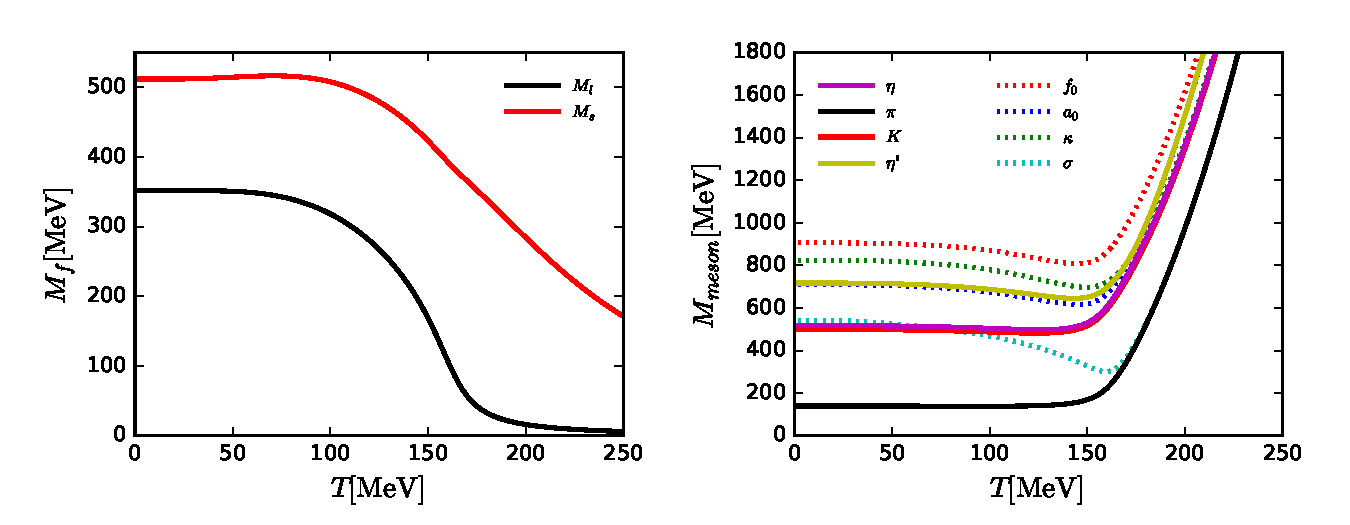
\includegraphics[width=0.95\textwidth]{MFMBO}
\caption{The quark (left panel) and meson masses (right panel) as functions of temperature at vanishing chemical potential. The solid and dashed lines in the right panel correspond to scalar and pseudoscalar meson fields, respectively.}\label{fig:MFMBO}
\end{figure*}
%%%%%%%%%%%%%%%%%%%%%%%%%%%%%
%

The meson fields are composite condensate fields from QCD theories. So we need to employ the Wetterich equation with dynamical hadronisation\cite{Fu:2019hdw}, which reads
\begin{align}\label{Wettericheq}
&\partial_t \Gamma_k[\Phi]+\int \langle  \partial_t  \hat \phi_{k,i}\rangle \bigg ( \frac{\delta \Gamma_k [\Phi]}{\delta \phi_i}+c_{\sigma_j} \delta_{i j}\bigg ) \\ \nonumber
&=\frac{1}{2} \text{Tr}(G_k[\Phi] \partial_t R_k)+\text{Tr}\bigg( G_{\phi \Phi_j} [\Phi] \frac{\delta \langle  \partial_t  \hat \phi_{k,i}\rangle}{\delta \Phi_j } R_{\phi} \bigg)
\end{align}
The flow of the chiral part of the effective potential reads
\begin{align}\label{eq:flowU}
\partial_t \tilde{U}_{k}(\Sigma,\Sigma^\dagger) &= \frac{k^4}{4 \pi^2}\bigg\{ \sum_i l_0^{(B,4)}(m_{i,k},\eta_\phi;T)\\ \nonumber
&-4 N_c( 2 l_0^{(F,4)}(m_{l,k},\eta_l;T,\mu)\\ \nonumber
& + l_0^{(F,4)}(m_{s,k},\eta_s;T,\mu)\bigg\}
\end{align}
The threshold functions $l_0^{(B/F,4)}$ are given in \app{app:loopfun}, The sum means all of the scalar and pseudoscalar nonets meson fields should be sum up.

We distinguish the light and strange dynamical hadronisation, which reads
\begin{align}
\langle  \partial_t  \hat \phi_{k}\rangle&= [(\bar q \dot{\pmb{A} }_{k}^{\frac{1}{2}} T_a  \dot{\pmb{A} }_{k}^{\frac{1}{2}}   q)+(\bar q \dot{\pmb{A} }_{k}^{\frac{1}{2}} i \gamma _5 T_a \dot{\pmb{A} }_{k}^{\frac{1}{2}} q)]+\dot{B}_k \Sigma
\end{align}
here $\dot{\pmb{A} }_{k}$ is also a diagonal matrix
\begin{align}
\dot{\pmb{A} }_{k}=\begin{pmatrix}
\dot{A}_{l,k}&0&0\\
0&\dot{A}_{l,k}&0\\
0&0&\dot{A }_{s,k}
\end{pmatrix}
\end{align}
As pointed out in ref \cite{Braun:2014ata, Fu:2019hdw} , we choose $\dot{B}_k =0$. For convenience, we introduce light and strange matrices $T^L$ and $T^S$, see \app{app:Yukawa_term}.
By taking the second derivative of $(\bar q T^a q)$ of each side of \Eq{Wettericheq}, we get
\begin{align}
- \partial_t \lambda_q + \dot{A}_{a,k} h_{k}=-\text{Flow} _{(\bar q T^a q) (\bar q T^a q)}^{(4)}
\quad \text{for} \quad a=L,S
\end{align}
Here, $\text{Flow} _{(\bar q T^a q) (\bar q T^a q)}^{(4)}$ denotes four-quark coupling flow equation. With the fully hadronised condition
\begin{align}\label{lambda_eq}
\lambda_q  \equiv 0 , \quad \forall k
\end{align}
we get the hadronisation function
\begin{align}
\dot{A}_{l,k}=-\frac{1}{ h_{l,k}} \text{Flow}_{(\bar q T^L q) (\bar q T^L q)}^{(4)} \\
\dot{A}_{s,k}=-\frac{1}{ h_{s,k}}  \text{Flow}_{(\bar q T^S q) (\bar q T^S  q)}^{(4)}
\end{align}
For the Yukawa couplings, we take the derivative of $(\bar q T^a q)$ of each side of \Eq{Wettericheq} and project it on light or strange part, we get
\begin{align}\label{Yukawa_eq}
\partial_t h_{l,k}&=-\frac{1}{\sigma_L} \frac{\delta {\tilde U}(\Sigma)}{\delta \bar \sigma_L}\dot{\bar A}_{l,k}+\frac{1}{ \sigma_L} \text{Re}  (\text{Flow} _{(\bar q T^L q)}^{(2)})\\
\partial_t h_{s,k}&=-\frac{1}{\sigma_S} \frac{\delta {\tilde U}(\Sigma)}{\delta \sigma_S}\dot{\bar A}_{s,k}+\frac{1}{ \sigma_S} \text{Re}  (\text{Flow}_{(\bar q T^S q)}^{(2)})
\end{align}
see \app{app:Yukawa_term} for more details.
%%%%%%%%%%%%%%%%%%%%%%%%%%%%%%%%%%%%%%%%%%%%%%%%%%%%%%%%%%%%%%%%%%%%%%%%%%
\section{Thermodynamical}
\label{sec:Thermodynamical}

Within the FRG framework, the pressure is given from the thermodynamical potential density
\begin{align}
p=\Omega(0,0)-\Omega(T,\mu)
\end{align}
with the thermodynamical potential density is the effective potential in the infrared
\begin{align}
\Omega(T,\mu)=\tilde{U}_{k}(\Sigma,\Sigma^\dagger)+U_{glue}(L,\bar L)
\end{align}
With the pressure, the free energy density reads
\begin{align}
\epsilon=-p+T s +\sum_{f=u,d,s} \mu_f n_f
\end{align}
here the entropy density and the quark number density are
\begin{align}\label{eq:entropy}
s=\frac{\partial p }{\partial T } \quad \quad n_f=\frac{\partial p}{\partial \mu_f}
\end{align}
We are interested in the interaction measure, i.e., the trace anomaly
\begin{align}
I=\epsilon - 3 p
\end{align}
for an idea gas, $I$ equal to zero. At vanishing chemical potential, it also has
\begin{align}\label{eq:trace}
I=T \frac{\partial}{\partial T} \bigg (\frac{p}{T^4} \bigg )
\end{align}
And the speed of sound at vanishing density squared \cite{Fu:2018qsk}
\begin{align}
{\tilde{c}_s}^2=\frac{s}{\partial \epsilon/\partial T}
\end{align}

The generalized susceptibilities of the baryon number are obtained from derivatives of the pressure
\begin{align}
\chi_n^B=\frac{\partial^n}{\partial (\hat \mu_B)^n}\frac{p}{T^4}
\end{align}
with $\hat \mu_B\equiv \mu_B/T$. The generalized susceptibilities are related with the cumulates of net baryon number probability distribution\cite{Luo:2017faz, Sun:2018ozp}, such as
\begin{align}
\chi_2^B=&\frac{1}{\mathcal{V}T^3}\langle (\delta N_B)^2 \rangle \\
\chi_4^B=&\frac{1}{\mathcal{V}T^3}\big(\langle (\delta N_B)^4 \rangle -3 \langle (\delta N_B)^2 \rangle ^2\big)\\
\chi_6^B=&\frac{1}{\mathcal{V}T^3}\big(\langle (\delta N_B)^6 \rangle -15 \langle (\delta N_B)^4 \rangle\langle (\delta N_B)^2 \rangle \\ \nonumber
&-10 \langle (\delta N_B)^3 \rangle^2 +30 \langle (\delta N_B)^2 \rangle^3 \big )
\end{align}
with $\delta N_B=N_B-\langle N_B \rangle$ and  volume $\mathcal{V}$. To get rid of the volume dependence, we introduce the ratio between the n-th and m-th order of the generalized susceptibilities, which are defined by
\begin{align}
R^B_{nm}=\frac{\chi_n^B}{\chi_m^B}
\end{align}
For hyper-order fluctuations studies within a PQM model, see \cite{Fu:2021oaw}


\section{Numerical results}
\label{sec:result}

\subsection{Numerical setup}

%
%%%%%%%%%%%%%%%%%%%%%%%%%%%%%
\begin{figure*}[t]
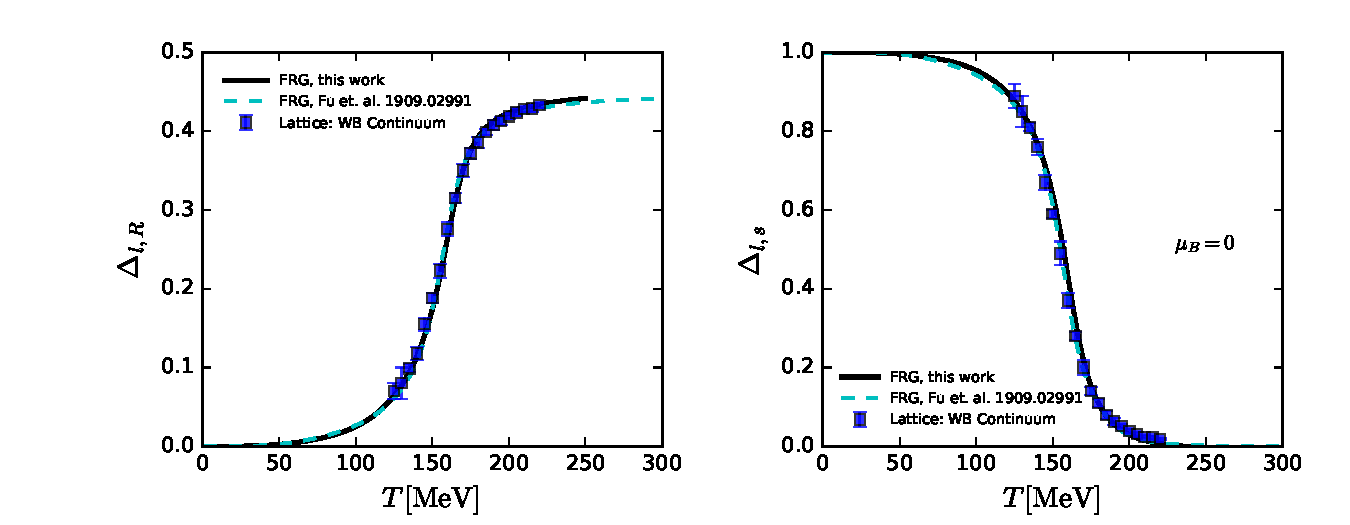
\includegraphics[width=0.95\textwidth]{Delta}
\caption{The renormalized light chiral condensate $\Delta_{l,R}$ (left panel) and  the reduced condensate $\Delta_{l,s}$ (right panel) . The former work result \cite{Fu:2019hdw} and lattice results by Wuppertal-Budapest collaboration \cite{Borsanyi:2010bp} }\label{fig:Delta}
\end{figure*}
%%%%%%%%%%%%%%%%%%%%%%%%%%%%%
%
We choose the UV cutoff $\Lambda=20$GeV. At this scale, only the strong coupling $\alpha_s$ and the current quark masses are fundamental couplings of QCD. We set the initial of the strong coupling as
\begin{align}
\alpha_{s,\Lambda}=0.235
\end{align}
which are same as $N_f=2+1$ case in \cite{Fu:2019hdw}. We employ a trivial initial effective potential
\begin{align}
\bar U_{k=\Lambda}(\rho_1,\rho_2)=\bar m_{\Lambda,\phi}^2 \bar \rho_1
\end{align}
with $\bar m_{\Lambda,\phi}^2=10^4\times\Lambda^2$ is square of the unique mesonic mass at UV scale. The input initial current quark masses are determined by the linear sigma terms, which are fixed by the vacuum pion mass $m_{\pi,k=0} = 138 \text{MeV}$, and the ratio of initial current quark masses $m_s^0/m_l^0=27$.  Then we arrived at
\begin{align}
c_l=3.5 \text{GeV}^3 \quad c_s=\frac{27}{\sqrt{2}} c_l
\end{align}
To compensate the missing nonclassical tensor structures, we use the infrared enhancement in \cite{Braun:2014ata,Fu:2019hdw}, The  enhancement strength parameter is adjusted to get the vacuum constituent light quark masses $m_{l,k=0}=350$MeV.

In \fig{fig:MFMBO} left panel, we show the light and strange quark masses as functions of temperature at vanishing chemical potential. At T=0, we set $m_{l,IR}=350$MeV and $m_{s,IR}=490$MeV.  At high temperature, the chiral symmetry is restored, the light quark mass trend to zero and the strange quark mass also declines. The pseudo critical temperature is around $150 \text{MeV}$, however,  a precise definition of the pseudo critical temperature is given by quark condensate, which will be shown later. In \fig{fig:MFMBO} right panel, we also show the masses of the nonets of scalar and pseudoscalar meson as functions of temperature. The solid and dashed lines correspond to scalar and pseudoscalar meson fields, respectively. At zero temperature, $m_ {\pi,IR}=138\text{MeV}$ , $m_{K,IR}=498 \text{MeV}$, $m_{\eta,IR}=543 \text{MeV}$ $\pi-\sigma$, $\eta' - a_0$, $\kappa-K$ are the chiral partners, which become degenerate with each other at high temperature. This  have been observed in low energy effective model \cite{Schaefer:2008hk,Tiwari:2013pg,Rai:2018ufz,Mitter:2013fxa,Rennecke:2016tkm,Wen:2018nkn}. One interesting thing is that in our theory, $\eta' - a_0$ are chiral partner, which is same with quark-meson model in mean-field approximation \cite{Schaefer:2008hk,Tiwari:2013pg,Rai:2018ufz} and LPA truncation\cite{Mitter:2013fxa,Rennecke:2016tkm,Wen:2018nkn} , rather than $\eta - a_0$, which is observed in quark-meson model beyond LPA truncation in  \cite{Rennecke:2016tkm}. This is related to the axial anomaly and the pseudoscalar mixing angles, a thorough analysis see  \cite{Rennecke:2016tkm}. Compared with the low energy effective theory results, meson masses in QCD increase faster at high temperature and the meson fields decouple faster from the system. This is also consistent with the result that the QCD chiral symmetry restore is stronger than the LEEF.

\subsection{Chiral condensates}

The chiral condensates are defined as
\begin{align}
\Delta_{q_i}=m_{q_i}^0\frac{T}{\mathcal{V}}\int_x\langle \bar q_i(x)q_i(x)\rangle
\end{align}
with volume $\mathcal{V}$ and no sum over the flavours index i is taken. To eradicate the volume factor and the renormalisation, it is common choice to calculate the renormalised condensate and the reduced condensate \cite{Fu:2019hdw}. The renormalised condensate is defined as
\begin{align}\label{eq:DeltaR}
\Delta_{q_i,R}=\frac{1}{\mathcal{N}_R}[\Delta_{q_i}(T,\mu_q)-\Delta_{q_i}(0,0)]
\end{align}
with $\mathcal{N}_R$ is a normalised constant.
The reduced condensate \cite{Herbst:2013ufa, Fu:2018qsk,Fu:2019hdw}
\begin{align}\label{eq:Deltals}
\Delta_{l,s}&\equiv\frac{\Delta_{l}(T,\mu_B)-\Big( \frac{m_l^0}{m_s^0} \Big)^2 \Delta_s(T,\mu_B)}{\Delta_{l}(0,0)-\Big( \frac{m_l^0}{m_s^0} \Big)^2 \Delta_s(0,0)}\\
&=\frac{\sigma_{l}(T,\mu_B)-\big( \frac{c_l}{c_s} \big) \sigma_s(T,\mu_B)}{\sigma_{l}(0,0)-\big( \frac{c_l}{c_s} \big) \sigma_s(0,0)}
\end{align}

In \fig{fig:Delta}, we plot the renormalised light chiral condensate $\Delta_{l,R}$ and  the reduced condensate $\Delta_{l,s}$ as functions of temperature  at vanished chemical potential. We compare with former work \cite{Fu:2019hdw}  and the lattice calculation \cite{Borsanyi:2010bp}. The the normalisation $\mathcal{N}_R$ in \Eq{eq:DeltaR} are same with the former work \cite{Fu:2019hdw}. Here we only choose the constituent quark mass $\Delta \bar m _{sl}=\bar m_s-\bar m_l=150 \text{MeV}$ results in \cite{Fu:2019hdw}, which corresponding the ratios of current quark mass $m_s^0/m_l^0=27$,   as comparison. Notable, in this work,  the constituent strange quark mass is self-consistent calculated  with  initial  condition $m_s^0/m_l^0=27$ . \fig{fig:Delta} show our results consistent well with the former work \cite{Fu:2019hdw}  and the lattice calculation \cite{Borsanyi:2010bp}.

The pseudo critical temperature is defined as the peak position of the renormalised light chiral condensate, $\partial t \Delta_{l,R}$. The pseudo critical temperature $T_c =156 \text{MeV}$, which is also in agreement with them. However, this is not a surprise, since one free parameter in the screening mass in the gluon propagator \cite{Fu:2019hdw} is employed to fix it.

\subsection{Equation of state}
\label{subsec:EoS}
%
%%%%%%%%%%%%%%%%%%%%%%%%%%%%%
\begin{figure*}[t]
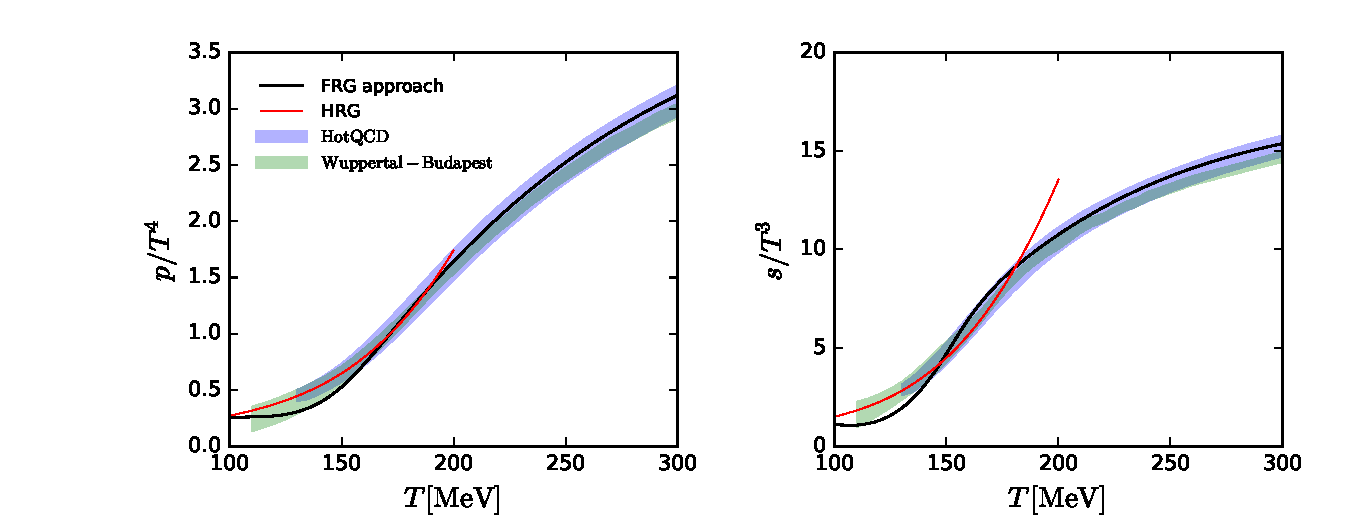
\includegraphics[width=0.95\textwidth]{P_s}
%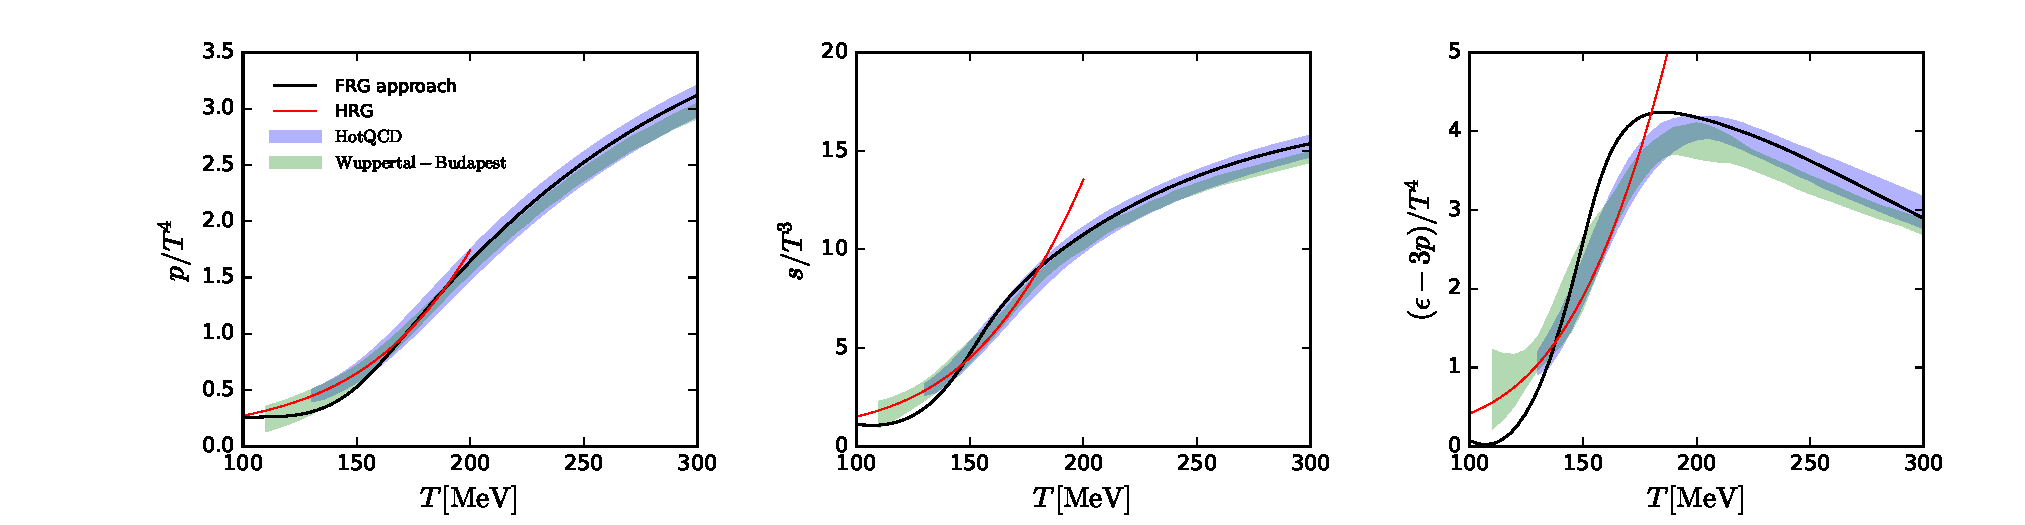
\includegraphics[width=1.\textwidth]{P_s_Tr}
\caption{The pressure (left panel) and entropy density (right panel) as functions of temperature at vanished chemical potential. We compared our results to the lattice results by HotQCD collaboration \cite{Bazavov:2014pvz} and by Wuppertal-Budapest collaboration \cite{Borsanyi:2013bia}. The HRG predictions are also plotted for comparison. }\label{fig:Pressure_entropy}
\end{figure*}
%%%%%%%%%%%%%%%%%%%%%%%%%%%%%
%

%
%%%%%%%%%%%%%%%%%%%%%%%%%%%%%
\begin{figure*}[t]
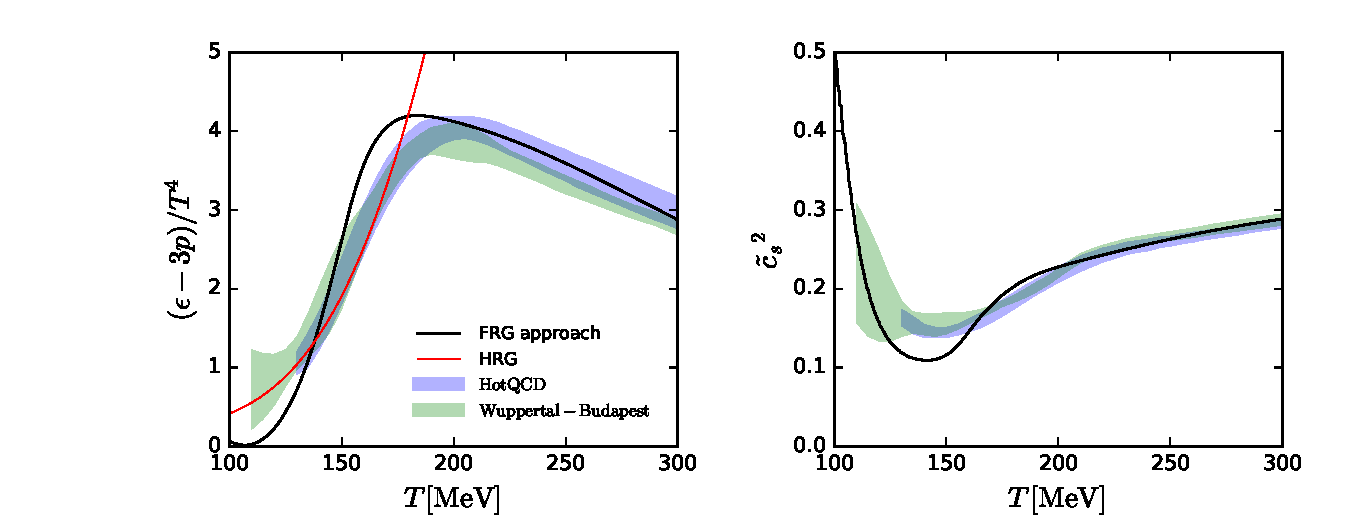
\includegraphics[width=0.95\textwidth]{Trace_Cs}
%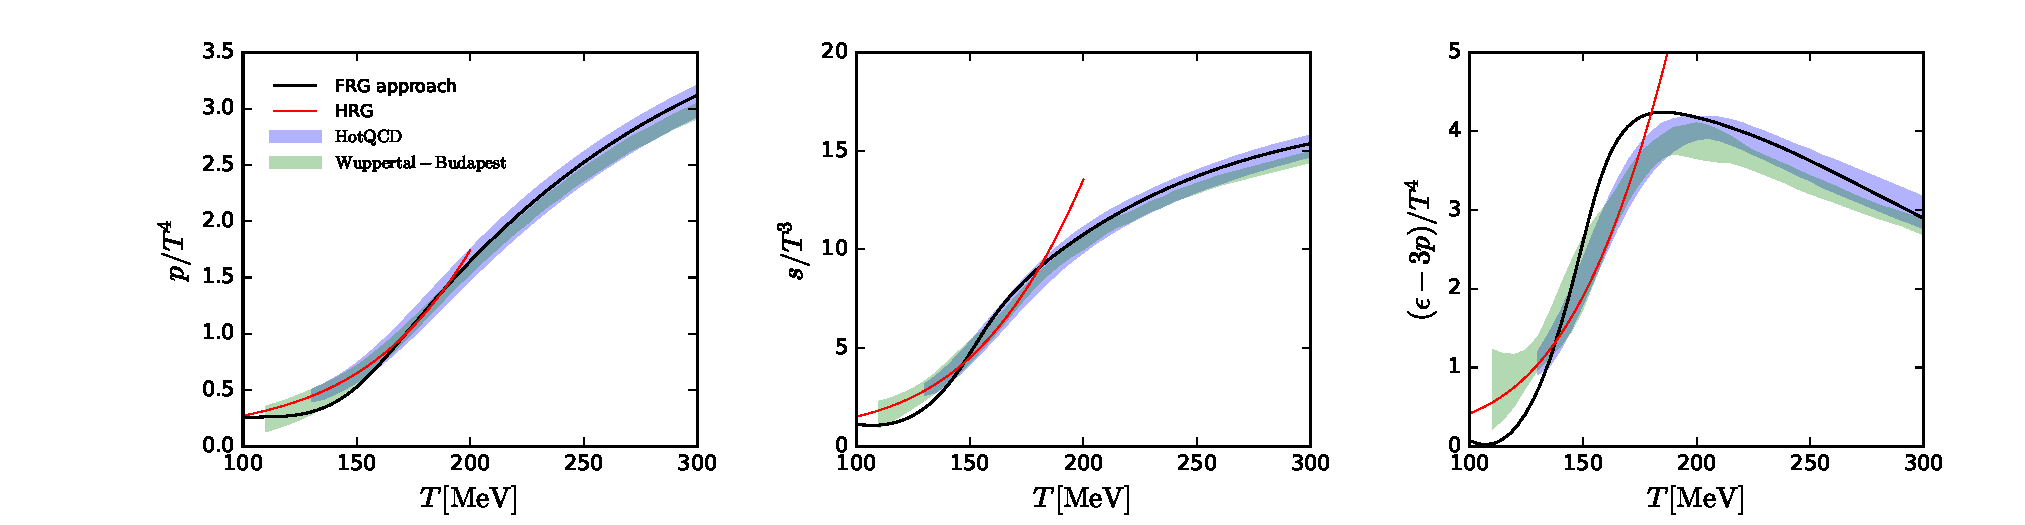
\includegraphics[width=1.\textwidth]{P_s_Tr}
\caption{The trace  anomaly (left panel) and  speed of sound (right panel) as functions of temperature at vanishing chemical potential. We compared our results to the lattice results by HotQCD collaboration \cite{Bazavov:2014pvz} and by Wuppertal-Budapest collaboration \cite{Borsanyi:2013bia}. The HRG predictions are also plotted for comparison. }\label{fig:Trace_Cs}
\end{figure*}
%%%%%%%%%%%%%%%%%%%%%%%%%%%%%
%

%
%%%%%%%%%%%%%%%%%%%%%%%%%%%%%
\begin{figure}[t]
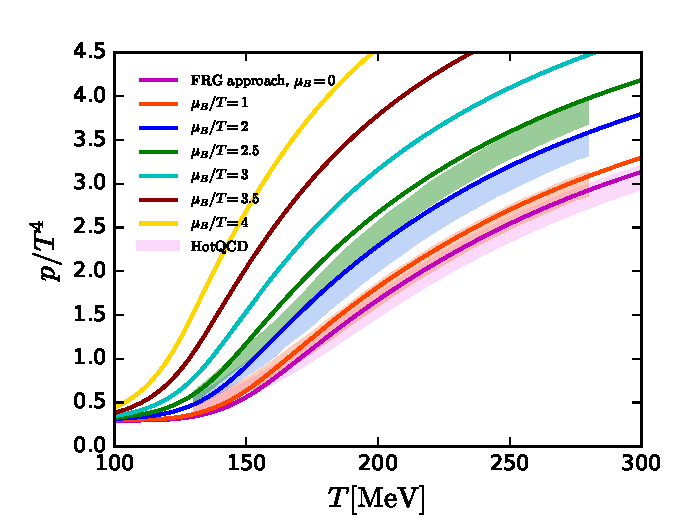
\includegraphics[width=0.5\textwidth]{Pressure_mu}
\caption{The pressure as functions of temperature at different chemical potential. We compared our results to the lattice results by HotQCD collaboration \cite{Bazavov:2017dus}. }\label{fig:Pressure_mu}
\end{figure}
%%%%%%%%%%%%%%%%%%%%%%%%%%%%%
%

%
%%%%%%%%%%%%%%%%%%%%%%%%%%%%%
\begin{figure*}[t]
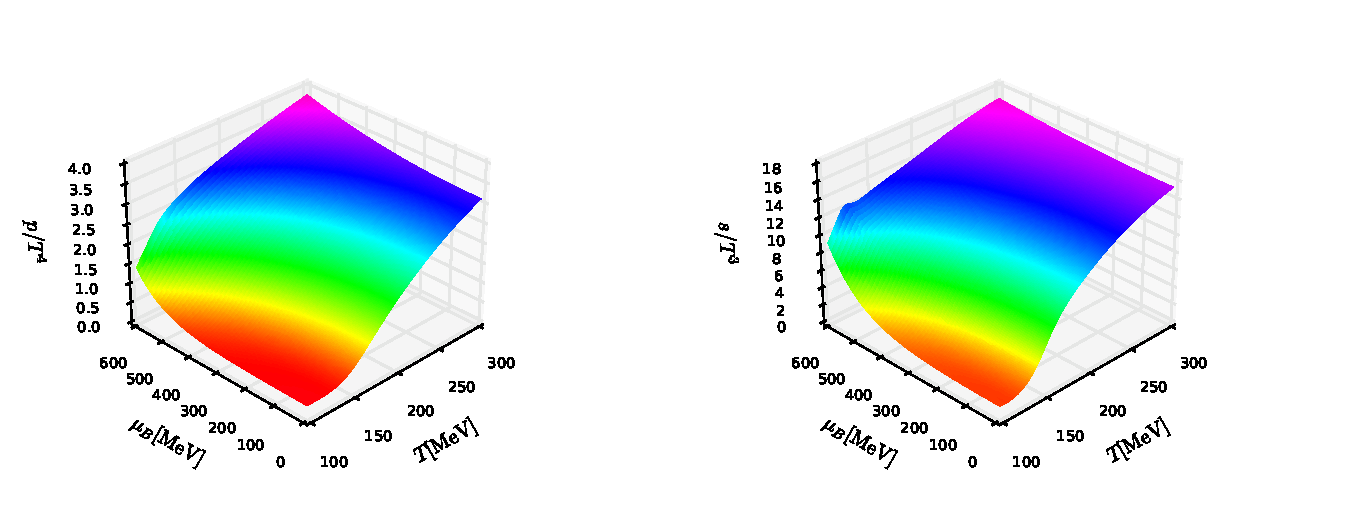
\includegraphics[width=1.\textwidth]{P_s_mu}
\caption{The pressure (left panel) and entropy density (right panel)  as functions of temperature and baryon number chemical potential. }\label{fig:P_s_mu}
\end{figure*}
%%%%%%%%%%%%%%%%%%%%%%%%%%%%%
%

In \fig{fig:Pressure_entropy}, we present the dimensionless pressure, entropy density and  the trace  anomaly as functions of temperature at vanished chemical potential. We compared them to the lattice results by HotQCD collaboration \cite{Bazavov:2014pvz} and by Wuppertal-Budapest collaboration \cite{Borsanyi:2013bia}. The hadron resonance gas (HRG) model, which are calculated from \cite{Vovchenko:2019pjl}, are also plotted for comparison.  To eradicate the unphysical temperature dependence of quark anomalous dimension $\eta_q$ at high scale $k$, we use a technical treatment, see in App. A more reasonable and self-consist treatment method is the two-loop frequency resummations which has been given in LEEF \cite{Fu:2016tey} and we will improve this part in the furture. As shown in \fig{fig:Pressure_entropy} left panel, the pressure is quantitative agreement with the lattice results. However, at low temperature, it is slight lower than the HRG model result. There has been a steady increase at $T \lesssim 130\text{MeV}$ and rapidly increase at  $T \sim 150\text{MeV}$ . It has been shown more clearly in entropy density in the middle and right panel of  \fig{fig:Pressure_entropy}, as it is the derivative of the pressure, see \Eq{eq:entropy}.  The entropy density is a little small at low temperature and  increase rapidly at $T\sim 150\text{MeV}$. The most likely causes of the concave of pressure at $T\sim  130 \text{MeV}$ is the parameterizations of Polyakov-loop potential, and a comparison of equation of state between different parameterizations of Polyakov-loop potential see \cite{Wen:2018nkn}. Otherwise, the entropy density from fRG approach is almost agreement with those of the lattice.

The higher order information of equation of state are presented in \fig{fig:Trace_Cs} and we also compare them with the lattice results and HRG model results. The trace anomaly and  the speed of sound from fRG approach are in qualitative, or even quantitative  agreement with those of the lattice results. However, the temperature corresponding to the peak of the trace anomaly is a bit lower than the lattice results. This also come from the concave of pressure and the reason have been analysed above. And it also cause the minimum value of speed of sound is lower than the lattice results. Besides, the speed of sound only have one minima in our calculation, which is much better than the LEEF results \cite{Fu:2018qsk}.

\fig{fig:Pressure_mu} presents the pressure at different $\mu_B/T$. We compare the results with the lattice results by HotQCD collaboration \cite{Bazavov:2017dus}, which are calculated using Taylor expansions in $\mu_B/T$ around vanishing $\mu_B$ with $\mu_S=\mu_Q=0$. At low chemical potential, our results are in good agreement with lattice results. Due to the sign problem and the convergency of the Taylor expansion, the lattice QCD cannot provide reliability pressure at $\mu_B/T>2.5$. Luckily, fRG approach does not suffer from those problems and can calculate it directly, and we predict the pressure at $\mu_B=3\sim4$. The pressure increase slowly with $\mu_B/T$ at low chemical potential and increase rapidly at high chemical potential. This can be easily understood in Taylor expansion form:
\begin{align}
\frac{p(T,\mu_B)-p(T,0)}{T^4}=&\frac{1}{2} \chi_2^B\Big(\frac{\mu_B}{T}\Big)^2+\frac{1}{4!}\chi_4^B\Big(\frac{\mu_B}{T}\Big)^4\\ \nonumber
&+\frac{1}{6!}\chi_6^B\Big(\frac{\mu_B}{T}\Big)^6+\cdots
\end{align}
Besides, we cannot see any concave of pressure around $T \sim 160 \text{MeV}$ at $\mu_B/T>2$, which is found in $\mathcal{O}(\mu_B^6)$ in \cite{Bazavov:2017dus}. This is caused by negative value of $\chi_6^B$, see \sec{subsec:B_fluctuations} , and can be compensated by higher order terms.

In \fig{fig:P_s_mu}, we plot 3D figures to present the pressure and entropy density as functions of temperature and baryon number chemical potential.The result are shown up to $\mu_B=600 \text{MeV}$, which is the maximum of out calculation due to the Taylor expansion method limit. The pressure is smoothly increased with the temperature and baryon number chemical potential, while  the entropy density has a non-monotonic behavior with temperature at high chemical potential in the neighborhood of CEP, which is not found in \cite{Parotto:2018pwx,Stafford:2021wik}. One of the possible causes of this is distinguishing of the chiral transition temperature and the de-confinement temperature at high chemical potential, see\cite{}.

\subsection{Baryon number fluctuations}
\label{subsec:B_fluctuations}
%
%%%%%%%%%%%%%%%%%%%%%%%%%%%%%
\begin{figure*}[t]
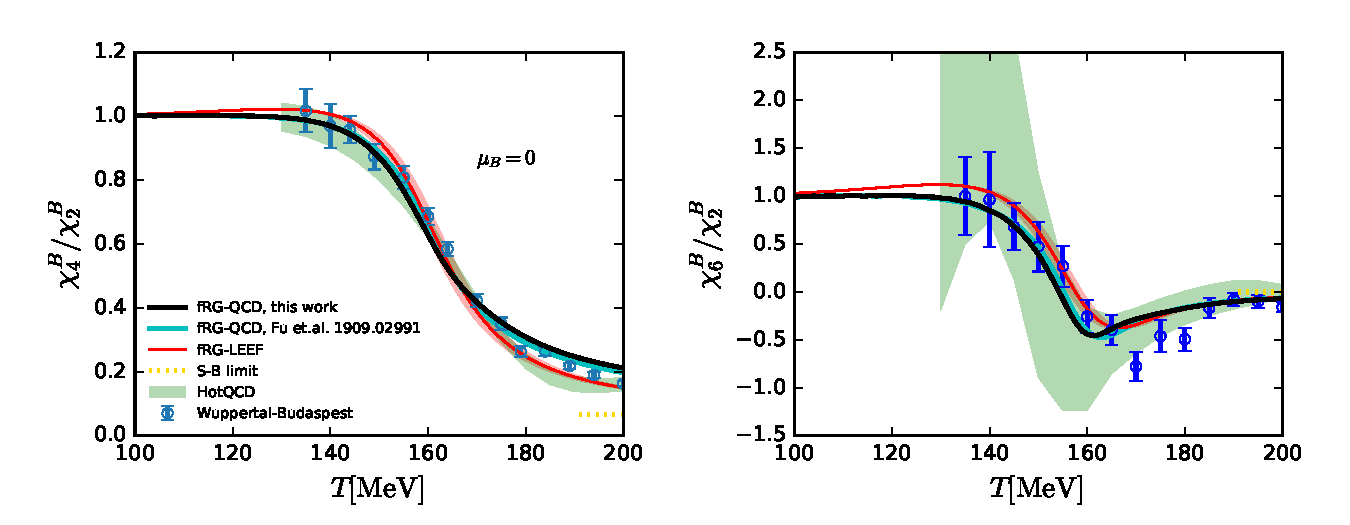
\includegraphics[width=0.95\textwidth]{M06mu0}
\caption{Ratios of baryon number fluctuations $R_{42}^B=\chi_4^B/\chi_2^B$ (left panel) and $R_{62}^B=\chi_6^B/\chi_2^B$ (right panel) as functions of temperature at vanished chemical potential. The lattice QCD results by the HotQCD collaboration \cite{Bazavov:2017tot} and the Wuppertal-Budapest collaboration \cite{Borsanyi:2018grb} are  plotted for comparison.  We also plot the rescaled LEEF results \cite{Fu:2021oaw} and QCD results calculated  from \cite{Fu:2019hdw} within fRG approach. The dashed yellow line denotes the  Stefan-Boltzmann limit.}\label{fig:R4262_mu0}
\end{figure*}
%%%%%%%%%%%%%%%%%%%%%%%%%%%%%
%
%
%%%%%%%%%%%%%%%%%%%%%%%%%%%%%
\begin{figure*}[t]
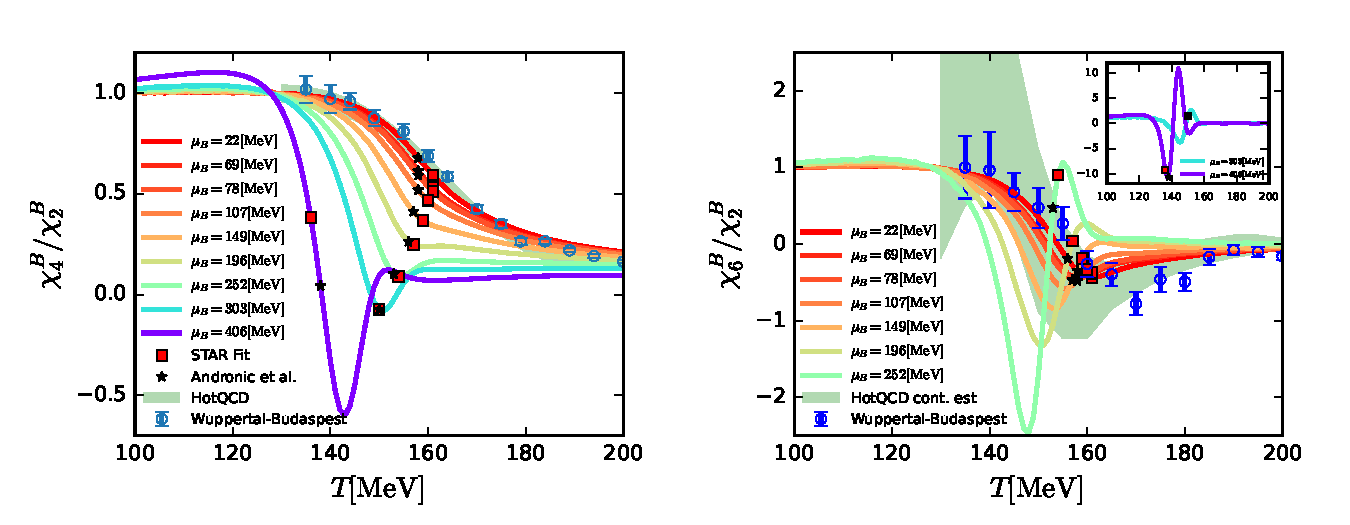
\includegraphics[width=0.95\textwidth]{M06mu}
\caption{Ratios of baryon number fluctuations $R_{42}^B=\chi_4^B/\chi_2^B$ (left panel) and $R_{62}^B=\chi_6^B/\chi_2^B$ (right panel) as functions of temperature at finite chemical potential. Square or star points denote different freeze-out scenarios, which are explain in the article. The lattice results at vanishing density are still plotted for comparison}\label{fig:R4262_mu}
\end{figure*}
%%%%%%%%%%%%%%%%%%%%%%%%%%%%%
%

%
%%%%%%%%%%%%%%%%%%%%%%%%%%%%%
\begin{figure}[t]
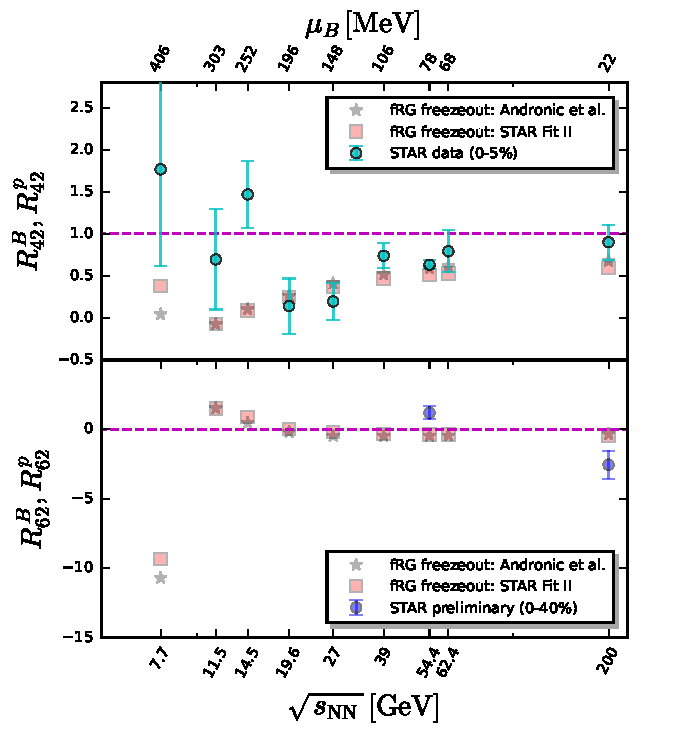
\includegraphics[width=0.48\textwidth]{R4262exp}
\caption{Ratios of baryon number fluctuations $R_{42}^B=\chi_4^B/\chi_2^B$ (left panel) and $R_{62}^B=\chi_6^B/\chi_2^B$ (right panel) as functions of collision energy. The STAR data from \cite{Adam:2020unf,Nonaka:2020crv,Pandav:2020uzx} are also plotted for comparison.}\label{fig:R4262_exp}
\end{figure}
%%%%%%%%%%%%%%%%%%%%%%%%%%%%%
%

In \fig{fig:R4262_mu0}, we depict the ratios of baryon number fluctuations as functions of temperature  at vanished chemical potential. We also compare our results with the lattice results \cite{Bazavov:2017tot,Borsanyi:2018grb} and rescaled PQM model results  \cite{Fu:2021oaw} with fRG approach. We also calculate baryon number fluctuations from the former work \cite{Fu:2019hdw}, which the $T_c^{glue}=250\text{MeV}$. Our results are also in good agreement with these results. At low temperature, the system close to a Skellam distribution which baryons and anti-baryons satisfy the Poisson distribution, and the ratio of fluctuations $R_{42}^B=R_{62}^B=R_{82}^B=\cdots=1$. With the temperature increase, the system take place a phase transition from confinement to deconfinement. At high temperature, it trends to the  Stefan-Boltzmann (SB) limit  i.e. $R_{42}^B=2/3\pi^2$, $R_{62}^B=0$ \cite{Fu:2009wy,Fu:2015naa}, also depicted in \fig{fig:R4262_mu0} . Besides, it exists a negative value in $R_{62}^B$ at $T\sim 160 \text{MeV}$, and the valley in QCD result is deeper than the LEEF result. Notable, no $R_{42}^B>1$ and $R_{62}^B>1$  at $T\sim 130 \text{MeV}$ are observed in our QCD results, which are observed in the LEEF results. This maybe an artifact in PQM model.

After comparing the baryon number fluctuations at vanished chemical potential, it allows us to predict the fluctuations at finite chemical potential in \fig{fig:R4262_mu}. Here we choose the freeze-out baryon number chemical potential from parameterizations of the collision energy in \cite{Andronic:2017pug}.
\begin{align}
\mu_{B_{CF}}=\frac{\alpha}{1+0.288\sqrt{s_{NN}}}
\end{align}
with $\alpha=1307.5\text{MeV}$. At low chemical potential, the ratio of fluctuations change slowly and close to the vanishing density results. The kurtosis drop at lower temperature with the chemical potential increasing, as both chiral and de-confinement temperature decrease with the chemical potential. At high $\mu_B  \sim$ 300 \text{MeV}, the kurtosis $R_{42}^B$ begin to $>1$ at low temperature and exist a negative value after the drop around the cross over temperature. And then it begin to exist a peek. The ratio $R_{62}^B$ have more complex structure at finite chemical potential and the amplitude of the ratio also increased. It begin to exit a peek at $\mu_B \gtrsim 150\text{MeV}$ and exit a second minima at $\mu_B\gtrsim400\text{MeV}$.

We also employ different freeze-out temperature scenarios, which are shown as square or star points  in \fig{fig:R4262_mu}. \colrui{The error bars are not taken into account in this work.} The red square point denote the parametrisation of the STAR data based on the four data points in $\mu_B=100\sim300\text{MeV}$ \cite{Fu:2021oaw} and the dark star point denote the parametrisation from \cite{Andronic:2017pug}, which reads
\begin{align}
T_{CF}=\frac{T_{CF}^{(0)}}{1+\exp(0.26-\ln(\sqrt{S_NN}/0.45))}
\end{align}
These results are also replotted in \fig{fig:R4262_exp}, which shows the $R_{42}^B$ and $R_{62}^B$ as functions of collision energy. The STAR data from \cite{Adam:2020unf,Nonaka:2020crv,Pandav:2020uzx} are also plotted for comparison. \cite{Abdallah:2021zhr} As we can see, the kurtosis $R_{42}^B$ and the hyper-kurtosis $R_{62}^B$ are non-monotonic dependence on the collision energy for both freeze-out scenarios, and different freeze-out scenarios have the same tendency. The kurtosis $R_{42}^B$ decline at low density and increase at high density, while the hyper-kurtosis $R_{62}^B$ increase at low density and decline at high density. Notable the tendency of the hyper-kurtosis $R_{62}^B$ is different from the LEEF results \cite{Fu:2021oaw}, and the non-monotonic behavior are far away form the CEP of our theory which located at $\mu_B \sim 635\text{MeV}$.
%%%%%%%%%%%%%%%%%%%%%%%%%%%%%%%%%%%%%%%%%%%%%%%%%%%%%%%%%%%%%



\section{Conclusions}
\label{sec:summary}

In this article, we extended the former work \cite{Fu:2019hdw} ��which includes the nonets of scalar and pseudoscalar mesons and self-consistently calculate the strange quark. The renormalized light chiral condensate $\Delta_{l,R}$ and the reduced condensate $\Delta_{l,s}$ are calculated to check our calculation. After that, we study the equation of state, such as pressure and entropy density, at vanishing and finite chemical potential. We also compare our results with the lattice QCD calculations at vanishing and finite chemical potential. Our results are in good agreement with them. We also calculate the ratios of baryon number fluctuations up to 6th order and compare them with lattice QCD results at vanishing chemical potential. Different freeze-out scenarios are employed which are mapping from the collision energy to the freeze-out temperature and chemical potential. And a non-monotonic dependence of the kurtosis on the collision energy is present.

This work is the first study of The equation of state and baryon number fluctuations in QCD theory within FRG approach. Some simplification and assumption have been employed and lots of things should be done in the future. The two-loop frequency resummations\cite{Fu:2016tey} should be done to eradicate the external frequency dependence and the quark loop cutoff in \app{app:loopfun}. Strangeness neutral and the fixed ratio of the electric charge to the baryon number density condition should be considered in the future. Fierz-complete four-quark interactions \cite{Braun:2017srn,Braun:2018bik,Braun:2019aow,Braun:2020mhk} and diquarks \cite{Fukushima:2021ctq} should be included to improve high density area and study the $U_A(1)$-symmetry.





%%%%%%%%%%%%%%%%%%%%%%%%%%%%%%%%%%%%%%%%%%%%%%%%%%%%%%%%%%%

\begin{acknowledgments}
%
We thank fQCD
%

\end{acknowledgments}

%%%%%%%%%%%%%%%%%%%%%%%%%%%%%%%%%%%%%%%%%%%%%%%%%%%%%%%%%%%%
%%%%%%%%%%%%%%%%%%%%%%%%%%%%%%%%%%%%%%%%%%%%%%%%%%%%%%%%%%%%%
	
\appendix

%%%%%%%%%%%%%%%%%%%%%%%%%%%%%%%%%%%%%%%%%%%%%%%%%%%%%%%%%%%%%%%%%	



\section{The Effective Potential and Meson masses}\label{app:mesonmass}

We perform the Taylor expansion of chiral symmetry invariant term in meson effective potential
\begin{align}
U_{k} (\rho_1,\rho_2)=\sum_{i,j=0}^{N_U} \frac{\lambda_{ij,k}}{i!j!}(\rho_1 -\kappa_{1,k})^i(\rho_2-\kappa_{2,k})^j
\end{align}
Here, we choose the expansion order $N_U=5$. $\kappa_{1,k}$,$\kappa_{2,k}$ are scale dependent expansion points, and we keep them always locating at  the minimum of the effective potential for every value of k. And the $\rho_1,\rho_2$ are defined as
\begin{align}
\rho_1&=\text{tr}(\Sigma \cdot \Sigma ^\dagger) \\
\rho_2&=\sqrt{6 \cdot \text{tr}\bigg (\Sigma \cdot \Sigma ^\dagger-\frac{1}{3} \rho_1 \mathbb{I}_{3 \times 3} \bigg )^2 }
\end{align}
At the vacuum expectation value (VEV) , $\rho_1,\rho_2$ are given as:
\begin{align}
\rho_1&=\frac{1}{2}(\sigma_l^2+\sigma_s^2)\\
\rho_2&=\frac{1}{2}(2 \sigma_s^2-\sigma_l^2)
\end{align}
Obviously, if the Taylor expansion converges, the physical observable should not depended on the expression basis, and we have checked that our expansion scenario converges well and it consists with other expression basis in \cite{Rennecke:2016tkm,Mitter:2013fxa}. However choosing a suitable basis can get concise mathematical expressions of meson masses and improve numerical stability.

The meson masses can be obtained from Hessian matrix \Eq{mesonmass_eq}, and theirs mathematical expression depended on the Taylor expansion basis \cite{Mitter:2013fxa,Rennecke:2016tkm}. The Hessian matrix of pseudoscalar in our Taylor expansion reads
\begin{align}
H_{p,LL}=&\frac{c_A \sigma_S}{\sqrt{2}}+U^{(1,0)}-U^{(0,1)}\\
H_{p,LS}=&\frac{c_A \sigma_L}{\sqrt{2}}\\
H_{p,SS}=&U^{(1,0)}+2 U^{(0,1)}\\
H_{p,11}=&-\frac{c_A \sigma_S}{\sqrt{2}}+U^{(1,0)}-U^{(0,1)}\\
H_{p,44}=&- \frac{c_A \sigma_L}{2} + U^{(1,0)} + \\ \nonumber
&\frac{\sigma_L^2- 3 \sqrt{2} \sigma_L \sigma_S+4 \sigma_S^2}{2 \sigma_S^2-\sigma_L^2} U^{(0,1)}\\
\end{align}
and for scalar
\begin{align}
H_{s,LL}=&-\frac{c_A \sigma_S}{\sqrt{2}}+U^{(1,0)}-U^{(0,1)} + \\ \nonumber
&(U^{(2,0)} -2U^{(1,1)}+U^{(0,2)})\sigma_L^2\\
H_{s,LS}=&-\frac{c_A \sigma_L}{\sqrt{2}}+ \\ \nonumber
&(U^{(2,0)}+U^{(1,1)}-2U^{(0,2)}) \sigma_L \sigma_S\\
H_{s,SS}=&U^{(1,0)}+2 U^{(0,1)} \\ \nonumber
&+(4 U^{(2,0)}+4U^{(1,1)}+U^{(2,0)})\sigma_S^2 \\
H_{s,11}=&\frac{c_A \sigma_S}{\sqrt{2}}+U^{(1,0)} +\frac{7 \sigma_L^2 - 2 \sigma_S^2}{2 \sigma_S^2-\sigma_L^2}U^{(0,1)}\\
H_{s,44}=&\frac{c_A \sigma_L}{2}+U^{(1,0)}+\\ \nonumber
&\frac{\sigma_L^2+3 \sqrt{2} \sigma_L\sigma_S+4 \sigma_S^2}{2 \sigma_S^2-\sigma_L^2}U^{(0,1)}
\end{align}
Because the nonvanishing nondiagonal element $H_{s/p,LS}$
we introduce the mixing angles between LS and physical basis:
\begin{align}\label{eq:plstrafo}
\begin{pmatrix}f_0 \\ \sigma \end{pmatrix} &= \begin{pmatrix} \cos\varphi_s & - \sin\varphi_s \\ \sin\varphi_s & \cos\varphi_s \end{pmatrix} \begin{pmatrix}\sigma_L \\ \sigma_S \end{pmatrix}\,,\\
\begin{pmatrix}\eta \\ \eta^\prime \end{pmatrix} &= \begin{pmatrix} \cos\varphi_p & - \sin\varphi_p \\ \sin\varphi_p & \cos\varphi_p \end{pmatrix} \begin{pmatrix}\eta_L \\ \eta_S \end{pmatrix}\,.
\end{align}
here
\begin{align}
\varphi_{s/p}=\frac{1}{2} arctan\Bigg(\frac{2H_{s/p,LS}}{H_{s/p,SS}-H_{s/p,LL}}\Bigg)
\end{align}
so the square of meson mass are given as
\begin{align}
m_{f_0}^2&=\cos^2\varphi_s H_{s,SS}+\sin^2 \varphi_s H_{s,LL}\\ \nonumber
&-2 \sin \varphi_s \cos \varphi_s H_{s,LS}\\
m_{\sigma}^2&=\sin^2\varphi_s H_{s,SS}+\cos^2 \varphi_s H_{s,LL}\\ \nonumber
&+2 \sin \varphi_s \cos \varphi_s H_{s,LS}\\
m_{a_0}^2&=H_{s,11}\\
m_{\kappa}^2&=H_{s,44}\\
m_{\eta}^2&=\cos^2\varphi_p H_{p,SS}+\sin^2 \varphi_p H_{p,LL}\\ \nonumber
&-2 \sin \varphi_p \cos \varphi_p H_{p,LS}\\
m_{\eta'}^2&=\sin^2\varphi_p H_{p,SS}+\cos^2 \varphi_p H_{p,LL}\\ \nonumber
&+2 \sin \varphi_p \cos \varphi_p H_{p,LS}\\
m_{\pi}^2&=H_{p,11}\\
m_{K}^2&=H_{p,44}
\end{align}
We can simplify them as
 \begin{align}
m_{f_0/\eta}^2=&\frac{H_{s/p,LL}+H_{s/p,SS}}{2}\\ \nonumber
&+\sqrt{(H_{s/p,LL}-H_{s/p,SS})^2+4 H_{s/p,LS}^2}\\
m_{\sigma/\eta'}^2=&\frac{H_{s/p,LL}+H_{s/p,SS}}{2}\\ \nonumber
&-\sqrt{(H_{s/p,LL}-H_{s/p,SS})^2+4 H_{s/p,LS}^2}
\end{align}

%%%%%%%%%%%%%%%%%%%%%%%%%%%%%%%%%%%%%%%%%%%%%%%%%%%%%%%%%%%%%%%%%%%%%
\section{Kobayashi-Maskawa-'t Hooft term}\label{app:tHooft_term}
The Kobayashi-Maskawa-'t Hooft coupling $\bar c_A$, which related with the $U_A(1)$ sysmmetry breaking, should decrease at high scalar and high temperatures. However, if we keep $c_A$ a constant, with
\begin{align}
\bar c_A=\frac{c_A}{Z_\phi^{3/2}}
\end{align}
$\bar c_A$ will increase with scalar and temperature. One scheme is given in ref \cite{Rennecke:2016tkm}, which assume that $\bar c_A$ is a constant. However, in this scheme, $U_A(1)$ symmetry can't restore at high scalar and it causes a very sharp phase transitions. In \cite{Li:2019chs}, they employ a temperature depended 't Hooft term, unfortunately, this leads to unphysical behavior of the pressure. We assume  $c_A$ is a infrared enhancement function
\begin{align}
c_A=c_{A,IR}\frac{1}{e^{\frac{k-k_{cut}}{\Delta_k}}+1}
\end{align}
here $k_{cut}=1.2 \text{GeV}$ and $\Delta_k=60 \text{MeV}$, $c_{A,IR}=$. And $\bar c_A$ still dressed as $\bar c_A=c_A/Z_\phi^{3/2}$. With these set,  $m_\eta=543 \text{MeV}$, which is close to $m_\eta=547\text{MeV}$ in PDG \cite{Zyla:2020zbs}. This set also guarantees that the 't Hooft term have no direct contribution to the pressure.

\section{Quarks anomalous dimension}\label{app:Quarks_anomalous}

We distinguish the light and strange quarks anomalous dimension, them can be calculate from the two-point functions with the lowest momentum and frequency \cite{Pawlowski:2014zaa,Fu:2015naa,Rennecke:2016tkm,Fu:2019hdw}
\begin{align}
\eta_{q_i}=\frac{1}{4 Z_{q_i,k}} \text{Re} \Bigg [ i \frac{\partial}{\partial |\vec{p}|^2} \text{tr} \vec \gamma \vec p \partial_t \Gamma_{\bar q_i q_i,k}^{(2)} (p) \Bigg ]_{\vec p=0}
\end{align}
with no sum over the flavours index $i$ is taken. Then we get the light quark anomalous dimension
\begin{align}
\eta_{l,k}=&\frac{1}{48 \pi^2} (4-\eta_{\phi,k})h_{l,k}^2 \Big [ 3 \mathcal {FB}_{(1,2)}(m_l,m_\pi)\\ \nonumber
&+3 \mathcal {FB}_{(1,2)}(m_l,m_{a_0})+\cos^2\varphi_s \mathcal {FB}_{(1,2)}(m_l,m_{f0})\\ \nonumber
&+\cos^2\varphi_p \mathcal {FB}_{(1,2)}(m_l,m_{\eta})+\sin^2\varphi_s \mathcal {FB}_{(1,2)}(m_l,m_{\sigma})\\ \nonumber
&+\sin^2\varphi_p \mathcal {FB}_{(1,2)}(m_l,m_{\eta'}) \Big]\\ \nonumber
&+\frac{1}{24 \pi^2} \frac{N_c^2-1}{2 N_c} g_{\bar q_l A q_l ,k}^2 \Big [ 2(4-\eta_{A,k})\mathcal {FB}_{(1,2)}(m_l,0)\\ \nonumber
&+3(3-\eta_{l,k})\big(\mathcal{FB}_{(1,1)}(m_l,0)-2 \mathcal{FB}_{(2,1)}(m_l,0)\big )\Big ]
\end{align}
and for the strange quark anomalous dimension
\begin{align}
\eta_{s,k}=&\frac{1}{24 \pi^2} (4-\eta_{\phi,k})h_{s,k}^2 \Big [\sin^2\varphi_s \mathcal {FB}_{(1,2)}(m_s,m_{f_0}) \\ \nonumber
&+\sin^2\varphi_p \mathcal {FB}_{(1,2)}(m_s,m_{\eta})+\cos^2\varphi_s \mathcal {FB}_{(1,2)}(m_s,m_{\sigma}) \\ \nonumber
&+\cos^2\varphi_p \mathcal {FB}_{(1,2)}(m_s,m_{\eta'}) \Big ]\\ \nonumber
&+\frac{1}{24 \pi^2} \frac{N_c^2-1}{2 N_c} g_{\bar q_s A q_s ,k}^2 \Big [ 2(4-\eta_{A,k})\mathcal {FB}_{(1,2)}(m_s,0)\\ \nonumber
&+3(3-\eta_{s,k})\big(\mathcal{FB}_{(1,1)}(m_s,0)-2 \mathcal{FB}_{(2,1)}(m_s,0)\big) \Big ]
\end{align}
for the fermion-boson mixed threshold function $\mathcal{FB}_{(i,j)}$ , see \cite{Fu:2019hdw}.

\section{Flow of the Yukawa couplings}\label{app:Yukawa_term}

The Yukawa couplings are renormalised as
\begin{align}
\bar h_{l/s}=\frac{h_{l/s}}{Z_\Sigma^{1/2} Z_{l/s}}
\end{align}
 Then, we rewrite the flow equation of Yukawa couplings \Eq{Yukawa_eq}.
\begin{align}
\partial_t \bar h_{l,k}=&\bigg(\eta_{l,k}+\frac{1}{2} \eta_{\phi,k}\bigg) - \frac{1}{\bar \sigma_L}\frac{\delta \bar { \tilde U}(\Sigma)}{\delta \bar \sigma_L} \dot{\bar A}_{l,k}\\ \nonumber
&+\frac{1}{\bar \sigma_L}\text{Re}\big(\overline{\text{Flow}}^{(2)}_{(\bar q T_L q)}\big) \\
\partial_t \bar h_{s,k}=&\bigg(\eta_{s,k}+\frac{1}{2} \eta_{\phi,k}\bigg) - \frac{1}{\bar \sigma_S}\frac{\delta \bar { \tilde U}(\Sigma)}{\delta \bar \sigma_S} \dot{\bar A}_{s,k}\\ \nonumber
&+\frac{1}{\bar \sigma_S}\text{Re}\big(\overline{\text{Flow}}^{(2)}_{(\bar q T_S q)}\big)
\end{align}
here
\begin{align}
T_L=\frac{1}{2}
\begin{pmatrix}
1& 0 & 0\\
0 & 1 & 0 \\
0 & 0 & 0
\end{pmatrix}
\quad
T_S=\frac{1}{\sqrt{2}}
\begin{pmatrix}
0& 0 & 0\\
0 & 0 & 0 \\
0 & 0 & 1
\end{pmatrix}
\end{align}
The coefficients before the dynamical hadronisation terms are given as
\begin{align}
\frac{1}{\bar \sigma_L} \frac{\delta \bar{\tilde U}(\Sigma)}{\delta \bar \sigma_L}&=- \frac{\bar c_A \bar \sigma_S}{\sqrt{2}} +\bar U^{(1,0)} -\bar U^{(0,1)}\\
\frac{1}{\bar \sigma_S} \frac{\delta \bar{\tilde U}(\Sigma)}{\delta \bar \sigma_S}&=- \frac{\bar c_A \bar \sigma_L^2}{2 \sqrt{2} \bar \sigma_S}+\bar U^{(1,0)} +2 \bar U^{(0,1)}
\end{align}
Notable,  the light coefficient $\frac{1}{\bar\sigma_L} \frac{\delta \bar{\tilde U}(\Sigma)}{\delta \bar \sigma_L}$ is also equal to $\bar m_\pi^2$, which is same with $N_f=2$ case.
The last term on the right hand side of \Eq{Yukawa_eq} reads
\begin{align}
\frac{1}{\bar \sigma_L}&\text{Re} ( \overline{\text{Flow}}_{(\bar q T_L q)}^{(2)})=
\frac{1}{8 \pi^2}\bar h_l^3\big [ 3 \mathcal{L}_{(1,1)}(m_l,a_0)\\ \nonumber
&-3 \mathcal{L}_{(1,1)}(m_l,\pi)+\cos^2 \varphi_s \mathcal{L}_{(1,1)}(m_l,f_0)\\ \nonumber
&-\cos^2 \varphi_p \mathcal{L}_{(1,1)}(m_l,\eta)+\sin^2 \varphi_s \mathcal{L}_{(1,1)}(m_l,\sigma)\\ \nonumber
&-\sin^2 \varphi_p \mathcal{L}_{(1,1)}(m_l,\eta')\\ \nonumber
&-\frac{3}{2 \pi^2} \frac{N_c^2-1}{2 N_c} g^2 _{\bar q_l A q_l} \bar h_l \mathcal{L}_{(1,1)}(m_l,0)
\end{align}
and for strange Yukawa coupling
\begin{align}
\frac{1}{\bar \sigma_S}&\text{Re} ( \overline{\text{Flow}}_{(\bar q T_S q)}^{(2)})=
\frac{1}{4 \pi^2}\bar h_s^3\big [ \sin^2 \varphi_s \mathcal{L}_{(1,1)}(m_l,f_0)\\ \nonumber
&-\sin^2 \varphi_p \mathcal{L}_{(1,1)}(m_l,\eta)+\cos^2 \varphi_s \mathcal{L}_{(1,1)}(m_l,\sigma)\\ \nonumber
&-\cos^2 \varphi_p \mathcal{L}_{(1,1)}(m_l,\eta')\\ \nonumber
&-\frac{3}{2 \pi^2} \frac{N_c^2-1}{2 N_c} g^2 _{\bar q_s A q_s} \bar h_s \mathcal{L}_{(1,1)}(m_s,0)
\end{align}

However, in our calculation, we only distinguish the glue sector of light and strange Yukawa couplings, and keep the meson sector of strange Yukawa coupling same with the light one. Because if we do so, the strange quark mass will lower than expect. This may because we keep the four-quark coupling flow function $\overline{\text{Flow}}_{(\bar l l)(\bar l l)}^4=\overline{\text{Flow}}_{(\bar s s)(\bar s s)}^4$ for simplify. And we will improve them in the further work.

\section{Polyakov-loop potential}

We employ the parameterizations Polyakov-loop potential from \cite{Lo:2013hla}, that is
\begin{align}
  \bar V_{\text{glue-Haar}} =& -\frac{\bar a(T)}{2} \bar L L + \bar b(T)\ln M_H(L,\bar{L})\\ \nonumber
  &+ \frac{\bar c(T)}{2} (L^3+\bar L^3) + \bar d(T) (\bar{L} L)^2
\end{align}
with
\begin{align}
M_H (L, \bar{L})&= 1 -6 \bar{L}L + 4 (L^3+\bar{L}^3) - 3  (\bar{L}L)^2\,.
\end{align}
for $x\in \{\bar a, \bar c, \bar d\}$
\begin{align}\label{eq:polyakov_xT}
  x(T) &= \frac{x_1 + x_2/(t+1) + x_3/(t+1)^2}{1 + x_4/(t+1) + x_5/(t+1)^2}
\end{align}
and
\begin{align}\label{eq:polyakov_bT}
  \bar b(T) &=\bar b_1 (t+1)^{-\bar b_4}(1 -e^{\bar b_2/(t+1)^{\bar b_3}} )
\end{align}
the coefficients are list in \Tab{tab:polyakov}

\begin{table}
  \centering
  \begin{tabular}{cccccc}
    \hline\hline
    & 1 & 2 & 3 & 4 & 5 \rule{0pt}{2.6ex}\rule[-1.2ex]{0pt}{0pt}
    \\ \hline
    $\bar a_i$ &-44.14& 151.4 & -90.0677 &2.77173 &3.56403 \\
    $\bar b_i$ &-0.32665 &-82.9823 &3.0 &5.85559  &\\
    $\bar c_i$ &-50.7961 &114.038 &-89.4596 &3.08718 &6.72812\\
    $\bar d_i$ &27.0885 &-56.0859 &71.2225 &2.9715 &6.61433\\\hline\hline
  \end{tabular}
  \caption{Parameterizations of Polyakov-loop potential in \Eq{eq:polyakov_xT} and \Eq{eq:polyakov_bT} .}\label{tab:polyakov}
\end{table}

The reduced temperature of QCD:
\begin{align}
  t_{\text{YM}}\rightarrow \alpha\,t_{\text{glue}},\quad
  t_{\text{glue}}\equiv(T-T_c^\text{glue})/T_c^\text{glue}
\end{align}
In this work, we choose
\begin{align}
T_c^{\text{glue}}=270 \text{[MeV]},\quad
\alpha=0.57
\end{align}

\section{loop function}\label{app:loopfun}


Here we give the loop funtion in the flow of effective potential \Eq{eq:flowU}. The bosonic loop reads
\begin{align}
l_0^{(B,4)}=\frac{1}{3}\Big(1-\frac{\eta_\phi}{5}\Big)\frac{k}{\sqrt{k^2+m_phi^2}}(1+2 n_B(m_\phi))
\end{align}
and the fermionic loop
\begin{align}
l_0^{(F,4)}=\frac{1}{3}\Big(1-\frac{\eta_q}{4}\Big)\frac{k}{\sqrt{k^2+m_q^2}}(1- n_F(m_q,\mu_B)-n_F(m_q,-\mu_B))
\end{align}
Here, $m_\phi$ and $m_q$ denote the meson and quark masses, and $n_B$ and $n_F$ denote the bosonic and fermionic distribution functions. As mentioned in \sec{subsec:EoS}, for scale $k>1.2\text{GeV}$, the zero order of fermionic loop function, we assume that
\begin{align}
l_0^{(F,4)}=\frac{1}{3}\Big(1-\frac{\eta_q}{4}\Big)\frac{k}{\sqrt{k^2+m_q^2}}(- n_F(m_q,\mu_B)-n_F(m_q,-\mu_B))
\end{align}
to eradicate the unphysical temperature dependence of quark anomalous dimension $\eta_q$ at high scale $k$.
%\
%\newpage
%\

%%%%%%%%%%%%%%%%%%%%%%%%%%%%%%%%%%%%%%%%%%%%%%%%%%%%%%%%%%%%%%%%
	
%\bibliography{refspec}% Produces the bibliography via BibTeX.
\bibliography{ref-lib}% Produces the bibliography via BibTeX.
	
	
\end{document}
